\section{The regularized model behind the simulations}\label[appendix]{app:regularized}

The simulations integrate the hyperviscous equation
\begin{equation}\label{eq:hyper}
\partial_tu+\mathcal P\bigl((u\cdot\nabla)u\bigr)+\nu\Lambda^2u+\mu\Lambda^{2\alpha}u=\mathcal Pf,
\qquad\Lambda=(-\Delta)^{1/2},
\end{equation}
on a periodic box, where the gradient part of a force $f$ is absorbed into the pressure, with $\mu=0$ in most runs and $\mu>0$ in the convergence check. This appendix
records what is known about \eqref{eq:hyper} at the scope used here. The proofs are analytic; the
Lean statements in \nolinkurl{Energy.lean}, \nolinkurl{Difference.lean} and \nolinkurl{Multiplier.lean}
only encode the abstract algebra noted below.

\begin{theorem}[Fixed-$\mu$ global regularity]\label{thm:hyper}
Let $\nu\ge0$, $\mu>0$ and $\alpha\ge5/4$. For smooth divergence-free initial data and smooth forcing,
\eqref{eq:hyper} has a unique global smooth solution.
\end{theorem}

This is the classical hyperviscous result \citep{lions1969quelques}. We use the critical energy
method of \citet[Section~2]{tao2009hyperdissipative}, adapted to the torus.

\noindent\emph{Reduction to zero mean.} The force enters only through $\mathcal Pf$, whose spatial mean
$\bar f(t)$ moves the mean velocity $m(t)=\overline{u_0}+\int_0^t\bar f$. With $X'(t)=m(t)$, $X(0)=0$, the
field $v(t,x)=u(t,x+X(t))-m(t)$ solves the same equation with zero-mean data and the zero-mean,
solenoidal force $\mathcal Pf(t,x+X(t))-\bar f(t)$. Translation preserves every Sobolev norm, and the
mean is controlled separately: $\|u(t)\|_{H^m}^2=\|v(t)\|_{H^m}^2+|\T^3|\,|m(t)|^2$. All estimates below
are for zero-mean $v$, which we again call $u$.

\noindent\emph{Local theory.} The semigroup $e^{-t(\nu\Lambda^2+\mu\Lambda^{2\alpha})}$ gains one derivative at
the cost $C(1+(\mu t)^{-1/(2\alpha)})$, which is integrable at $t=0$ because $1/(2\alpha)<1$. The
Duhamel map is therefore a contraction in $C([0,\delta];H^m)$, $m\ge3$, so a uniform $H^m$ bound
before a putative maximal time allows a restart beyond it.

\noindent\emph{Energy.} Nonlinear cancellation and Young's inequality give
$\|u(t)\|_{L^2}^2+\mu\int_0^t\|\Lambda^\alpha u\|_{L^2}^2\le\|u_0\|_{L^2}^2+\mu^{-1}\int_0^t\|\Lambda^{-\alpha}f\|_{L^2}^2$,
so $a(t)=\|\Lambda^{5/4}u(t)\|_{L^2}$ is square-integrable on every finite interval.

\noindent\emph{Higher energy.} After differentiating $m$ times, the top transport term cancels. Every
remaining term has the form $\int(\nabla^ju)(\nabla^{j_1}u)(\nabla^{j_2}u)$ with $j_1+j_2=j+1$.
The finite-exponent embeddings $\|\nabla u\|_{L^{12/5}}\lesssim\|\Lambda^{5/4}u\|_{L^2}$ and
$\|\nabla^ju\|_{L^{12}}\lesssim\|\Lambda^{5/4}\nabla^ju\|_{L^2}$, Gagliardo--Nirenberg interpolation and
H\"older bound these terms by $C_m\,a(t)\,\|u\|_{H^m}\,\|\Lambda^\alpha u\|_{H^m}$. Absorbing half of
the dissipation gives
$X'\le(1+C_m\mu^{-1}a(t)^2)X+\|f\|_{H^m}^2$ for $X=\|u\|_{H^m}^2$. The coefficient is integrable,
so Gr\"onwall bounds $X$ on every finite interval.

\noindent The constants degenerate as $\mu\to0$. The theorem says nothing about $\mu=0$.

\begin{theorem}[Conditional recovery at rate $O(\mu)$]\label{thm:recovery}
Fix $\nu>0$, $\alpha\ge5/4$ and common smooth data and forcing. Suppose the Navier--Stokes solution
$v$ ($\mu=0$) is smooth on a given interval $[0,T]$, and let $u_\mu$ be the solution of \eqref{eq:hyper}.
For every integer $m\ge3$ there are $K_m$ and $\mu_m>0$, depending on $v$, $T$, the box, $m$,
$\alpha$ and $\nu$ but not on $\mu$, such that
\[
\sup_{0\le t\le T}\|u_\mu(t)-v(t)\|_{H^m}\le K_m\,\mu\qquad\text{for }0<\mu\le\mu_m .
\]
\end{theorem}

\begin{proof}[Sketch]
The difference $w=u_\mu-v$ starts at zero and satisfies
$\partial_tw+\nu\Lambda^2w+\mu\Lambda^{2\alpha}w+B(v,w)+B(w,v)+B(w,w)=-\mu\Lambda^{2\alpha}v$, where
$B(a,b)=\mathcal P((a\cdot\nabla)b)$. The regularization acts as dissipation on $w$ plus a source
that depends only on the smooth reference. Transport cancellation, product estimates and
$H^m\subset W^{1,\infty}$ give
$\tfrac12X'\le C_m(M+\sqrt X)X+\mu F\sqrt X$ for $X=\|w\|_{H^m}^2$, $M=\sup_{[0,T]}\|v\|_{H^{m+1}}$ and
$F=\|\Lambda^{2\alpha}v\|_{H^m}$. While $X\le1$ this becomes $X'\le A_mX+\mu^2F^2$, so
$X(t)\le\mu^2K_m^2$ with $K_m^2=e^{A_mT}\int_0^TF^2$. For $\mu\le\mu_m=1/(2\max(1,K_m))$ this keeps
$X\le1/4$, so the region $X\le1$ is never left. No bound on $u_\mu$ uniform in $\mu$ is assumed; the
bootstrap produces it.
\end{proof}

The rate uses reference regularity $H^{m+2\alpha}$. Smoothness of $v$ on $[0,T]$ is a premise. The
theorem gives no continuation of Navier--Stokes beyond $T$. In Lean, \nolinkurl{inner_rhs_self_le_zero}
and the \nolinkurl{Difference.lean} lemmas prove the abstract energy and difference-energy algebra
in a real inner-product space. The Sobolev estimates and the bootstrap are not mechanized.

\paragraph{Numerical check.}
On a fixed $24^3$ grid with $\nu=10^{-3}$ and $\alpha=2$, the relative low-mode difference between
the $\mu>0$ run and the $\mu=0$ run, measured on the modes with $|k|\le4$ at $t=0.1$, decreases with $\mu$ (\cref{fig:mu-convergence}).
This is a finite-dimensional consistency check on one grid. It does not supply the smooth reference
of \cref{thm:recovery}.

\begin{figure}[t]
  \centering
  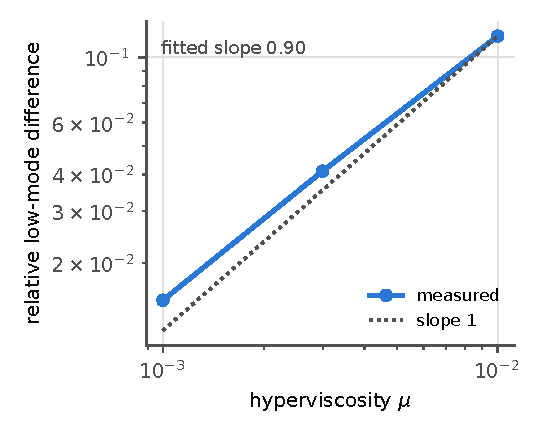
\includegraphics[width=0.55\linewidth]{figures/mu_convergence.pdf}
  \caption{\textbf{Fixed-grid convergence in $\mu$.} Relative low-mode difference between the
  hyperviscous run and the $\mu=0$ run on the same $24^3$ grid at $t=0.1$, for three values of
  $\mu$. The dotted line has slope one; the least-squares slope over the three points is 0.90.}
  \label{fig:mu-convergence}
\end{figure}

\paragraph{A remark on low-frequency closure.}
The Six Birds packaging step suggests replacing the eliminated scales by an effective linear term.
Suppose that term is a scalar, isotropic, time-local symbol $\ell(|k|^2)$ acting on solenoidal fields,
with $\ell$ twice differentiable near zero, $\ell(0)=0$ and $\ell(r)\ge0$ for all small $r>0$. Then
$\ell'(0)\ge0$ (\nolinkurl{viscosity_coeff_nonneg}) and Taylor's formula gives
$\ell(r)=\ell'(0)\,r+O(r^2)$. In an equation that already contains $\nu\Lambda^2$, the leading
coefficient becomes $\nu+\ell'(0)$. Three caveats apply. The coefficient $\ell'(0)$ can vanish, as
for $\ell(r)=r^2$. Positivity at the lattice frequencies of a fixed box does not imply positivity
near zero: $\ell(r)=r^2-r/2$ is positive at every $r=|k|^2\ge1$ but has $\ell'(0)=-1/2$, and Lean
proves this counterexample (\nolinkurl{fixed_mode_passivity_counterexample}). And an autonomous
lift of a memory equation is local in the enlarged state, not in the velocity alone, so it does not
supply the time-local premise. The actual bridge of \cref{def:bridge} keeps its full history.
